\documentclass{article}

\usepackage{algorithmic}
\usepackage{amsmath}
\usepackage{graphicx}
\usepackage{hyperref}
\usepackage{booktabs}
\usepackage{verbatim}

\begin{document}

\title{SVM Handwriting Classification\\
       Midterm Exam}
\author{Geoffrey Ulman\\
        CSI747}
\date{October 2012}
\maketitle

\section{Primal Soft-Margin SVM}\label{model1}

The primal soft-margin SVM classifier was built using the optimization problem in Equation \ref{svm1}.

\begin{equation}\label{svm1}
\begin{split}
\min 0.5\left( \vec{w} \cdot \vec{w} \right) + C \sum_{i=1}^l \xi_i \\
s.t. \\
\xi_i \ge 0 \\
y_i \left( \left( \vec{x_i} \cdot \vec{w} \right) - b \right) \ge 1 , i = 1,2,...,l
\end{split}
\end{equation}

\subsection{Primal Soft-Margin AMPL Model}

\begin{verbatim}

model;

# lines in file (number of training images)
param l;

# pixels per image (size of training vector)
param n;

# weight on xi penalty coefficient in primal problem
param C;

# output vector (1 or -1)
param y { 1..l };

# input data
param x { 1..l, 1..n };

# hyperplane parameters
var w { 1..n };
var b;

# relaxation allowing for non-separable problems
var xi { 1..l };

minimize obj: 0.5 * ( sum { i in 1..n } w[i]^2 ) +
                C * ( sum { i in 1..l } xi[i] ) ;

s.t. nonneg { i in 1..l }: xi[i] >= 0;

s.t. hplane { i in 1..l }: y[i] *
              ( ( sum { k in 1..n }
                   x[i,k] * w[k] ) - b ) >= 1 - xi[i] ;

option solver loqo;

\end{verbatim}

\subsection{Primal Soft-Margin Results}

\begin{verbatim}

LOQO 6.07: optimal solution (18 QP iterations, 18 evaluations)
primal objective 3.808456385
  dual objective 3.808456358

"option abs_boundtol 2.8429960302606307e-10;"
will change deduced dual values.

w [*] :=
 1 -3.15451e-27   17  1.82133e-10   33 -0.111267      49 -0.0343738
 2  0.118075      18  0.14054       34 -0.301305      50  0.0933198
 3  0.213456      19 -0.0293014     35 -0.442642      51  0.000171579
 4  0.0818948     20 -0.0770882     36 -0.0416026     52 -0.402848
 5  0.0715085     21  0.741797      37  0.0835767     53 -0.0667686
 6  0.0349342     22  0.501937      38  0.0884881     54  0.0430135
 7 -0.0338163     23  0.198454      39 -0.232727      55  0.0195015
 8 -3.15451e-27   24 -0.131832      40 -0.00596055    56 -0.00596055
 9  8.52162e-11   25 -0.111267      41 -0.129117      57  0.0910099
10  0.339545      26 -0.259003      42 -0.631474      58 -0.0155056
11  0.348543      27 -0.217968      43 -0.662013      59  0.0763903
12  0.475353      28 -0.111734      44 -0.151043      60  0.0520377
13  0.000296062   29  0.285148      45  0.0745046     61 -0.240032
14  0.0637961     30  0.328823      46 -0.232932      62  0.037993
15  0.0661811     31  0.179537      47 -0.187038      63  0.148775
16 -3.15451e-27   32 -3.15451e-27   48  0.0581445     64 -3.15451e-27
;

xi [*] :=
  1 3.54215e-10    48 4.28256e-10    95 3.68708e-10   142 3.775e-10
  2 0.463301       49 3.71314e-10    96 3.76266e-10   143 7.32662e-10
  3 1.49441        50 0.0323216      97 0.0920738     144 3.40313e-10
  4 4.08089e-10    51 3.83008e-10    98 0.072318      145 3.31577e-10
  5 4.00877e-10    52 3.89458e-10    99 3.7132e-10    146 4.24756e-10
  6 3.67217e-10    53 3.36558e-10   100 1.84125       147 0.59652
  7 1.20085        54 3.87526e-10   101 1.1496        148 4.18158e-10
  8 3.88911e-10    55 4.30938e-10   102 3.60704e-10   149 3.97591e-10
  9 0.214791       56 0.41072       103 0.00359628    150 4.38972e-10
 10 1.28133e-08    57 4.1869e-10    104 3.91538e-10   151 4.03546e-10
 11 3.94828e-10    58 3.16047e-10   105 2.21851e-09   152 0.565352
 12 3.77228e-10    59 3.90868e-10   106 4.3815e-10    153 0.894454
 13 1.39793e-09    60 2.843e-10     107 4.12031e-10   154 0.375176
 14 3.46076e-10    61 1.6605e-08    108 4.11394e-10   155 3.85445e-10
 15 3.90668e-10    62 3.95981e-10   109 3.07597e-08   156 3.8433e-10
 16 3.89596e-10    63 3.38845e-10   110 0.135305      157 4.00168e-10
 17 3.84253e-10    64 0.263084      111 3.85553e-10   158 4.20697e-10
 18 3.78775e-10    65 7.81376e-10   112 3.71473e-10   159 3.79116e-10
 19 4.17314e-10    66 0.402768      113 4.2554e-10    160 3.89053e-10
 20 3.87605e-10    67 3.44195e-10   114 3.831e-10     161 0.143884
 21 4.04914e-10    68 3.35975e-10   115 3.93818e-10   162 0.199411
 22 3.74905e-10    69 0.662451      116 3.27886e-10   163 4.35077e-10
 23 0.0274426      70 3.82252e-10   117 4.22175e-10   164 4.1439e-10
 24 0.231874       71 3.98174e-10   118 0.140067      165 3.32473e-10
 25 4.19624e-10    72 0.145354      119 0.127478      166 3.72152e-10
 26 1.2731         73 0.945562      120 3.7356e-10    167 6.75207e-10
 27 3.26029e-10    74 0.256505      121 4.11598e-10   168 0.34252
 28 3.88575e-10    75 5.01638e-10   122 3.75389e-10   169 0.575049
 29 8.17445e-10    76 3.87452e-10   123 3.1802e-10    170 4.11112e-10
 30 3.87155e-10    77 1.10393e-07   124 4.17731e-10   171 3.17172e-10
 31 3.61122e-10    78 3.27744e-10   125 4.31632e-10   172 3.99229e-10
 32 7.53563e-10    79 4.31609e-08   126 4.18139e-10   173 3.65298e-10
 33 3.5612e-10     80 3.43132e-10   127 0.911277      174 3.34136e-10
 34 4.35504e-10    81 4.26958e-10   128 3.56167e-10   175 5.7491e-10
 35 3.97985e-09    82 3.73867e-10   129 3.55418e-10   176 0.228682
 36 4.1976e-10     83 0.52189       130 3.69854e-10   177 3.81167e-10
 37 3.87513e-10    84 4.06703e-10   131 3.62618e-10   178 3.75641e-10
 38 1.02411e-08    85 3.83031e-10   132 3.84984e-10   179 0.191379
 39 3.8985e-10     86 3.66646e-10   133 4.17247e-10   180 0.447845
 40 1.84448e-09    87 3.77081e-10   134 2.82501e-09   181 1.42038e-09
 41 4.14366e-10    88 0.846396      135 4.24345e-10   182 3.75385e-10
 42 3.65064e-10    89 1.41052       136 8.34873e-10   183 4.10451e-10
 43 3.91127e-10    90 4.08348e-10   137 4.32896e-10   184 3.636e-10
 44 4.277e-10      91 4.05179e-10   138 3.55676e-09   185 1.45174e-09
 45 4.25439e-10    92 4.19322e-10   139 1.16151       186 4.51322e-10
 46 4.04992e-10    93 4.10816e-10   140 4.31328e-10
 47 0.0204862      94 4.02686e-10   141 3.93777e-10
;

b = 0.0120722

\end{verbatim}

Java was used to parse the AMPL results and the input data files. The hyperplane defined by \(\vec{w}\) and \(b\) was then used to classify the testing data and calculate the misclassification error rate. The following Java snippet calculates the classifier output \(y\) for a set of test data (data parsing and support code omitted for brevity):

\begin{verbatim}

public static double[] calculate_y_predicted_primal(
                            List<TrainingExample> dataListTest,
                            List<TrainingExample> dataListTrain,
                            OutputGenerator out, double[] w, double b )
{
    double[] y_predicted = new double[dataListTest.size( )];

    // iterate over the training examples
    for ( int i = 0; i < dataListTest.size( ); i++ )
    {
        TrainingExample x_i = dataListTest.get( i );

        double sum = 0;
        double[] x = x_i.getInputs( );
        for ( int j = 0 ; j < x.length ; j++ )
        {
            sum += x[j] * w[j];
        }

        y_predicted[i] = sum - b;
    }

    return y_predicted;
}

\end{verbatim}

The penalty constant \(C\) was set to \(0.1\) after testing a series of values, running the classifier, and observing the training error. Figure \ref{cvserror} shows the improvement of the testing data error rate as \(C\) approaches \(0.1\).

\begin{figure}\label{cvserror}
\centering
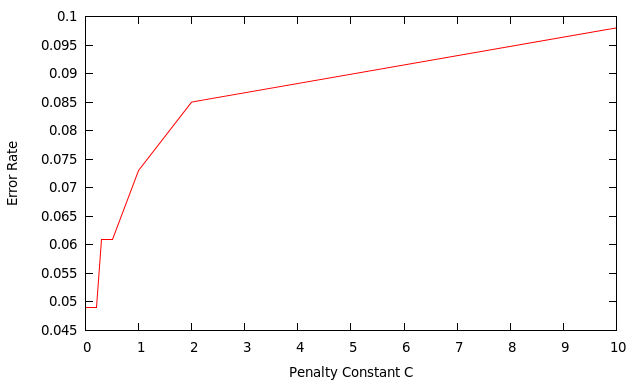
\includegraphics[width=0.9\textwidth]{dual_c_vs_error_rate.png}
\caption{Primal Penality Constant Versus Error Rate}
\end{figure}

\begin{table}\label{table1}
\caption{Primal Soft-Margin Digit 3 vs 6 Error}
\begin{center}
\begin{tabular}{llcc}
\toprule
Data Set & Error & \multicolumn{2}{c}{95\% Confidence Interval} \\
\cmidrule(r){3-4}
& & Lower Bound & Upper Bound \\
\midrule
Training & 0.038 & 0.010 & 0.065 \\
Testing & 0.049 & 0.002 & 0.095 \\
\bottomrule
\end{tabular}
\end{center}
\end{table}

Table \ref{table1} indicates that the primal soft-margin SVM classifier perfectly classified the training data set and acheived a \(0.049\) misclassification error rate for the testing data set for digits ''3`` and ''6``.

\section{Dual Soft-Margin SVM}\label{model2}

The dual soft-margin SVM classifier was built using the optimization problem in Equation \ref{svm2}.

\begin{equation}\label{svm2}
\begin{split}
\max \sum_{i=1}^l \alpha_i - 0.5 \sum_{i,j}^l \alpha_i \alpha_j y_i y_j \left( \vec{x_i} \cdot \vec{x_j} \right) \\
s.t. \\
0 \ge \alpha_i \ge C , i = 1,2,...,l \\
\sum{i=1}^l \alpha_i y_i = 0 , i = 1,2,...,l
\end{split}
\end{equation}

\subsection{Dual Soft-Margin AMPL Model}

\begin{verbatim}

model;

# lines in file (number of training images)
param l;

# pixels per image (size of training vector)
param n;

# weight on xi penalty coefficient in primal problem
param C;

# output vector (1 or -1)
param y { 1..l };

# input data
param x { 1..l, 1..n };

# dual problem variables and simple constraints
var a { 1..l } >= 0, <= C ;

maximize obj: ( sum { i in 1..l } a[i] ) - 0.5 * sum { i in 1..l, j in 1..l } ( a[i] * a[j] * y[i] * y[j] * sum { k in 1..n } ( x[i,k] * x[j,k] ) ) ;

s.t. const: sum { i in 1..l } a[i] * y[i] = 0 ;

option solver loqo;

\end{verbatim}

\subsection{Dual Soft-Margin Results}

\begin{verbatim}

LOQO 6.07: optimal solution (24 QP iterations, 24 evaluations)
primal objective 3.80845635
  dual objective 3.8084564
a [*] :=
  1 9.08547e-10    48 9.32775e-11    95 7.93618e-11   142 2.44836e-10
  2 0.1            49 9.12306e-10    96 4.20253e-10   143 0.0401223
  3 0.1            50 0.1            97 0.1           144 7.69043e-10
  4 1.2248e-10     51 1.31798e-10    98 0.1           145 1.81561e-09
  5 9.73511e-11    52 1.30999e-10    99 0.0119755     146 1.19908e-10
  6 4.27862e-10    53 2.61964e-09   100 0.1           147 0.1
  7 0.1            54 1.2823e-10    101 0.1           148 2.10874e-10
  8 2.09772e-10    55 8.28051e-11   102 1.58991e-09   149 1.23291e-10
  9 0.1            56 0.1           103 0.0999983     150 9.75451e-11
 10 0.0825943      57 1.39014e-10   104 4.12959e-10   151 1.69916e-10
 11 1.52064e-10    58 7.97273e-10   105 0.0700139     152 0.1
 12 1.1513e-10     59 1.02462e-10   106 1.41395e-10   153 0.1
 13 0.064105       60 4.79618e-08   107 1.2443e-10    154 0.1
 14 3.18092e-10    61 0.090468      108 2.16825e-10   155 1.82193e-10
 15 1.68031e-10    62 1.43344e-10   109 0.0896112     156 5.54399e-10
 16 4.6803e-10     63 2.35787e-09   110 0.1           157 1.47753e-10
 17 5.46372e-10    64 0.1           111 0.0179415     158 3.02381e-10
 18 5.45239e-10    65 0.0437021     112 9.37855e-11   159 2.65331e-10
 19 3.3423e-10     66 0.1           113 1.54081e-10   160 3.81309e-10
 20 1.16503e-10    67 6.13164e-09   114 2.23757e-10   161 0.1
 21 8.35008e-11    68 2.57918e-09   115 2.49166e-10   162 0.1
 22 8.02316e-11    69 0.1           116 3.75511e-09   163 9.7388e-11
 23 0.1            70 4.9684e-10    117 9.24059e-11   164 2.17704e-10
 24 0.1            71 4.38411e-10   118 0.1           165 0.0135987
 25 9.85652e-11    72 0.1           119 0.1           166 5.83863e-10
 26 0.1            73 0.1           120 6.04793e-10   167 0.0325091
 27 1.1187e-09     74 0.1           121 1.17864e-10   168 0.1
 28 0.00971835     75 0.050468      122 1.48579e-10   169 0.1
 29 0.0495885      76 0.0180752     123 7.44134e-09   170 0.0182398
 30 2.73722e-10    77 0.0947431     124 1.73175e-10   171 5.85755e-09
 31 7.17799e-10    78 3.29336e-09   125 1.91625e-10   172 8.09361e-11
 32 0.0255155      79 0.0942866     126 2.17789e-10   173 4.83287e-10
 33 1.56251e-09    80 3.20645e-08   127 0.1           174 8.49808e-10
 34 1.18584e-10    81 1.96128e-10   128 4.13511e-10   175 0.0318319
 35 0.0770716      82 9.77418e-10   129 7.37342e-10   176 0.1
 36 2.19962e-10    83 0.1           130 5.11948e-10   177 4.68524e-10
 37 1.19845e-10    84 1.50151e-10   131 8.73983e-10   178 3.90043e-10
 38 0.0910098      85 1.09665e-10   132 2.72968e-10   179 0.1
 39 1.56061e-10    86 1.0144e-09    133 7.22915e-11   180 0.1
 40 0.0661812      87 1.32879e-09   134 0.0721417     181 0.0625603
 41 1.32986e-10    88 0.1           135 9.82361e-11   182 2.544e-10
 42 5.83862e-10    89 0.1           136 0.0445782     183 1.22333e-10
 43 9.79412e-11    90 1.80474e-10   137 1.97218e-10   184 1.73124e-09
 44 1.8122e-10     91 8.51483e-11   138 0.067866      185 0.0666886
 45 1.19837e-10    92 1.05237e-10   139 0.1           186 1.00778e-10
 46 1.60272e-10    93 1.42097e-10   140 1.73984e-10
 47 0.1            94 0.0178502     141 1.16911e-10
;

\end{verbatim}

The value of \(b\) was calculated for all support vectors (those with \(0 < \alpha_i < C\)) as a check on the correctness of the solution. The table below displays the calculated \(b\) values for each such \(\alpha\). The final \(b\) value used in the classification of the testing data was the average of these \(b\) values.

\begin{verbatim}

#alpha index, alpha value, calculated b
6 0.5531 0.188856798305
8 0.3733 0.188861160199
9 0.0029 0.188871934348
12 0.0531 0.188864376841
18 0.0393 0.188854459866
22 0.0602 0.188871164725
25 0.4170 0.188862548853
27 0.2798 0.188865861802
28 0.5098 0.188865357024
34 0.7256 0.188849350391
37 0.1898 0.188853567449
46 0.1669 0.188858772546
48 0.2942 0.188851064662
52 0.5802 0.188862980571
55 0.7082 0.188853273441
63 0.3538 0.188866929197
68 0.6685 0.188871266426
72 0.8144 0.188867736297
73 0.1018 0.188857462442
77 0.0754 0.188856395052
87 0.0556 0.188872370964
96 0.1804 0.188853107931
97 0.5155 0.188852990917
100 0.4256 0.188855950912
102 0.0825 0.188854038379
104 0.1136 0.188870270977
115 0.5621 0.188873322808
118 0.0967 0.188872624401
126 0.7636 0.188865448670
130 0.1043 0.188856390173
133 0.0968 0.188847704220
138 0.7243 0.188857459050
142 0.0527 0.188860768228
146 0.2022 0.188850473924
151 0.4116 0.188865036435
152 0.8614 0.188865290240
153 0.4057 0.188868509620
160 0.5062 0.188870428611
164 0.6873 0.188869861530
168 0.7740 0.188854538469
169 0.1119 0.188854672264
179 0.1979 0.188858462089
184 0.1469 0.188857771249

\end{verbatim}

\begin{table}\label{table2}
\caption{Dual Soft-Margin Digit 3 vs 6 Error}
\begin{center}
\begin{tabular}{llcc}
\toprule
Data Set & Error & \multicolumn{2}{c}{95\% Confidence Interval} \\
\cmidrule(r){3-4}
& & Lower Bound & Upper Bound \\
\midrule
Training & 0.038 & 0.010 & 0.065 \\
Testing & 0.049 & 0.002 & 0.095 \\
\bottomrule
\end{tabular}
\end{center}
\end{table}

Table \ref{table2} indicates that the dual soft-margin SVM classifier perfectly classified the training data set and acheived a \(0.049\) misclassification error rate for the testing data set for digits ''3`` and ''6``. This is identical to the results achieved for the primal problem (which makes sense because the formulations should be equivalent). The same penality constant value \(C=0.1\) was the best value for the dual problem as well as the primal problem.

\section{Dual Polynomial SVM}\label{model3}

The dual polynomial SVM classifier was built using the optimization problem in Equation \ref{svm3}.

\begin{equation}\label{svm3}
\begin{split}
\max \sum_{i=1}^l \alpha_i - 0.5 \sum_{i,j}^l \alpha_i \alpha_j y_i y_j \left( \alpha \left( \vec{x_i} \cdot \vec{x_j} \right) + \beta \right)^d \\
s.t. \\
0 \ge \alpha_i \ge C , i = 1,2,...,l \\
\sum{i=1}^l \alpha_i y_i = 0 , i = 1,2,...,l
\end{split}
\end{equation}

\subsection{Dual Polynomial AMPL Model}

\begin{verbatim}

model;

# lines in file (number of training images)
param l;

# pixels per image (size of training vector)
param n;

# weight on xi penalty coefficient in primal problem
param C;

# polynomial machine kernel parameters
param alpha;
param beta;
param delta;

# output vector (1 or -1)
param y { 1..l };

# input data
param x { 1..l, 1..n };

# dual problem variables and simple constraints
var a {1..l} >= 0, <= C;

maximize obj: sum { i in 1..l } a[i] -
              0.5 * sum { i in 1..l, j in 1..l }
                           a[i] * a[j] * y[i] * y[j] * ( alpha * (
                           sum { k in 1..n } x[i,k] * x[j,k] ) + beta ) ^ delta;

s.t. const: sum { i in 1..l } a[i] * y[i] = 0;

option solver loqo;

\end{verbatim}

\subsection{Dual Polynomial Results}

\begin{verbatim}

LOQO 6.07: optimal solution (22 QP iterations, 22 evaluations)
primal objective 2867.882418
  dual objective 2867.882425
a [*] :=
  1   1.02531e-07    48   8.61577e-09    95   2.10839e-08   142   1.48999e-08
  2  98.4474         49   4.61188e-07    96  34.9011        143  27.6442
  3 100              50  30.4183         97  37.7857        144   4.66503
  4   6.5328e-08     51   1.86643e-06    98  10.8704        145   2.7213e-08
  5   1.2032e-07     52   1.11213e-07    99  25.9701        146   1.4305e-08
  6  12.9816         53  97.8993        100 100             147  25.5623
  7  28.3116         54   4.77467e-08   101  23.6605        148   9.86569e-09
  8   6.33472e-08    55   7.64781e-09   102   2.27673e-08   149   1.32595e-08
  9  44.7894         56   8.51246       103   5.24267e-07   150   2.33402e-08
 10  26.3581         57   1.39012e-08   104  10.3686        151   1.542e-08
 11  36.7381         58   4.29743e-07   105  39.3451        152   2.82917
 12   1.07092e-07    59   2.05962e-08   106   4.16072e-07   153 100
 13  74.2736         60 100             107   2.71187e-08   154 100
 14  11.9111         61   8.48449e-08   108   4.24606       155  39.1819
 15   1.82933e-08    62   3.15818e-08   109 100             156   8.86615
 16   1.35129e-07    63  16.6566        110  36.8726        157   3.07667e-08
 17  41.4348         64  63.5389        111  53.4906        158   1.05893e-07
 18  20.8818         65  36.6983        112   7.23013       159   2.16737e-05
 19   4.30859e-06    66 100             113  19.614         160   3.15004e-08
 20   3.23797        67   0.000156624   114  10.0767        161  67.9115
 21   1.43615e-08    68  89.4563        115 100             162   1.16297e-07
 22 100              69 100             116 100             163   8.37258e-09
 23 100              70   2.0411e-08    117   8.08354e-09   164   1.87303e-08
 24 100              71   1.68419e-08   118 100             165  22.6818
 25   1.75544e-08    72  36.2032        119 100             166  96.2878
 26 100              73  52.5948        120  67.3897        167   1.95622e-07
 27 100              74  59.7171        121 100             168  57.8253
 28  40.8574         75   2.47863       122   2.3803e-08    169  17.8739
 29 100              76  15.1736        123  25.873         170   6.14482
 30   2.16068e-07    77   3.22647e-06   124   7.29567e-08   171   1.25933
 31   2.03066e-06    78  49.6606        125   4.94565e-08   172   1.04854e-07
 32   3.85756e-08    79   8.19333       126  48.5045        173   9.48377e-08
 33  59.5537         80   1.37222       127 100             174  18.5993
 34   1.50233e-08    81   4.01854e-08   128   1.81162e-07   175  37.0473
 35   1.54028e-07    82   4.6698e-08    129  37.4749        176 100
 36   1.62842e-08    83  40.1234        130   5.07964e-08   177   2.07399e-08
 37   1.49206e-08    84   3.85788e-08   131  34.2697        178   3.55846e-08
 38  16.7662         85  51.4942        132   7.80473e-08   179 100
 39   1.98667e-08    86  17.3654        133   6.14671e-09   180 100
 40   2.53905e-07    87  81.9708        134   2.76429e-08   181  73.9895
 41   0.103716       88 100             135   1.61786e-08   182   4.9928e-08
 42   5.10616e-08    89 100             136   2.2634e-07    183   1.38181e-08
 43   3.01842e-08    90   4.56927e-08   137   1.14858e-08   184   5.57055e-07
 44   1.19128e-08    91   1.29279e-08   138   2.34395e-08   185  25.356
 45   1.11601e-08    92   9.98219       139  82.4303        186   1.12149e-08
 46   2.1805e-08     93  12.6638        140   1.308e-08
 47  13.8354         94  68.5562        141   1.34735e-08
;

\end{verbatim}

The value of \(b\) was calculated for all support vectors (those with \(0 < \alpha_i < C\)) in the same manner as for the dual soft-margin problem in Section \ref{model2}.

\begin{verbatim}

#alpha value, calculated b
98.4474 0.003688057498
12.9816 0.003688219777
28.3116 0.003689360280
44.7894 0.003688990222
26.3581 0.003688019794
36.7381 0.003689233929
74.2736 0.003688981995
11.9111 0.003688561909
41.4348 0.003689095055
20.8818 0.003689023799
3.2380 0.003688472784
40.8574 0.003688865371
59.5537 0.003688906990
16.7662 0.003688761357
0.1037 0.003695737907
13.8354 0.003688425517
30.4183 0.003688270055
97.8993 0.003688426899
8.5125 0.003688976897
16.6566 0.003689144953
63.5389 0.003689011298
36.6983 0.003688580128
89.4563 0.003688441483
36.2032 0.003688147806
52.5948 0.003688233328
59.7171 0.003689335758
2.4786 0.003688938989
15.1736 0.003689095760
49.6606 0.003688668794
8.1933 0.003688627345
1.3722 0.003688150932
40.1234 0.003689538042
51.4942 0.003688334140
17.3654 0.003688354074
81.9708 0.003688425479
9.9822 0.003688209154
12.6638 0.003687213091
68.5562 0.003688553410
34.9011 0.003690060290
37.7857 0.003690222677
10.8704 0.003691053320
25.9701 0.003689453009
23.6605 0.003688199671
10.3686 0.003689730633
39.3451 0.003689168432
4.2461 0.003689282127
36.8726 0.003688797655
53.4906 0.003688706942
7.2301 0.003688278618
19.6140 0.003687876768
10.0767 0.003687977832
67.3897 0.003688923886
25.8730 0.003688569845
48.5045 0.003689123141
37.4749 0.003688113516
34.2697 0.003689853627
82.4303 0.003688933590
27.6442 0.003690255237
4.6650 0.003689246088
25.5623 0.003689210145
2.8292 0.003689643357
39.1819 0.003689726944
8.8662 0.003689347001
67.9115 0.003688349042
22.6818 0.003688557541
96.2878 0.003688524804
57.8253 0.003689285044
17.8739 0.003688683644
6.1448 0.003689311403
1.2593 0.003688751264
18.5993 0.003689598874
37.0473 0.003688764178
73.9895 0.003688189170
25.3560 0.003688246100

\end{verbatim}

\begin{table}\label{table3}
\caption{Dual Polynomial Digit 3 vs 6 Error}
\begin{center}
\begin{tabular}{llcc}
\toprule
Data Set & Error & \multicolumn{2}{c}{95\% Confidence Interval} \\
\cmidrule(r){3-4}
& & Lower Bound & Upper Bound \\
\midrule
Training & 0.000 & 0.000 & 0.000 \\
Testing & 0.037 & -0.004 & 0.077 \\
\bottomrule
\end{tabular}
\end{center}
\end{table}

Table \ref{table3} indicates that the dual polynomial SVM classifier perfectly classified the training data set and acheived a \(0.037\) misclassification error rate for the testing data set for digits ''3`` and ''6`` with penalty constant \(C=100\).

\section{Dual Radial SVM}\label{model4}

The dual radial SVM classifier was built using the optimization problem in Equation \ref{svm4}.

\begin{equation}\label{svm4}
\begin{split}
\max \sum_{i=1}^l \alpha_i - 0.5 \sum_{i,j}^l \alpha_i \alpha_j y_i y_j e^{-\gamma \| x - x_i \|^2 } \\
s.t. \\
0 \ge \alpha_i \ge C , i = 1,2,...,l \\
\sum{i=1}^l \alpha_i y_i = 0 , i = 1,2,...,l
\end{split}
\end{equation}

\subsection{Dual Radial AMPL Model}

\begin{verbatim}

model;

# lines in file (number of training images)
param l;

# pixels per image (size of training vector)
param n;

# weight on xi penalty coefficient in primal problem
param C;

# parameters for radial basis function kernel
param gamma;

# output vector (1 or -1)
param y { 1..l };

# input data
param x { 1..l, 1..n };

# dual problem variables and simple constraints
var a {1..l} >= 0, <= C;

maximize obj: sum { i in 1..l } a[i] -
              0.5 * sum { i in 1..l, j in 1..l }
                      ( a[i] * a[j] * y[i] * y[j] * exp( -gamma * ( 
                      sum { k in 1..n } ( ( x[i,k] - x[j,k] )^2 ) ) ) );

s.t. const: sum { i in 1..l } a[i] * y[i] = 0;

option solver loqo;

\end{verbatim}

\subsection{Dual Radial Results}

\begin{verbatim}

LOQO 6.07: optimal solution (20 QP iterations, 20 evaluations)
primal objective 53.83866255
  dual objective 53.83866423
a [*] :=
  1 0.0835205      48 1.08389e-08    95 3.95684e-09   142 1.1919e-08
  2 1.68979        49 0.721593       96 0.750603      143 1.1128
  3 2              50 1.10289        97 1.62747       144 0.280222
  4 6.86854e-09    51 0.0999029      98 0.469429      145 1.10932e-08
  5 8.39209e-09    52 5.7903e-09     99 1.0157        146 5.18126e-09
  6 0.644339       53 0.804181      100 2             147 2
  7 1.74816        54 9.62904e-09   101 2             148 1.91219e-08
  8 1.86438e-08    55 4.49558e-09   102 4.82231e-08   149 6.80483e-09
  9 1.83991        56 1.36479       103 0.923025      150 8.22023e-09
 10 0.630288       57 6.4741e-09    104 2.37255e-07   151 2.63974e-08
 11 0.310396       58 0.64683       105 0.614093      152 1.55237
 12 8.46713e-09    59 5.99453e-09   106 1.07806e-08   153 2
 13 1.3559         60 1.28657       107 7.64931e-09   154 2
 14 5.8915e-08     61 0.12706       108 3.36592e-06   155 1.59631e-08
 15 6.95535e-09    62 7.21003e-09   109 5.67999e-08   156 0.290096
 16 0.0708219      63 0.315678      110 1.38359       157 5.62945e-09
 17 0.80453        64 1.54286       111 0.892388      158 1.35452e-08
 18 0.0250783      65 1.02985e-07   112 1.06861e-08   159 0.149991
 19 3.38021e-08    66 2             113 4.38241e-08   160 0.000973461
 20 1.09657e-08    67 3.23285e-08   114 0.249086      161 1.37089
 21 4.44345e-09    68 4.86676e-08   115 1.0861e-08    162 0.11776
 22 3.55428e-09    69 2             116 1.15512       163 6.12141e-09
 23 0.591677       70 1.76405e-08   117 5.17798e-09   164 1.79269e-07
 24 0.934571       71 4.15716e-07   118 0.294603      165 0.839991
 25 4.08618e-09    72 1.33675       119 1.81976       166 0.107207
 26 2              73 2             120 5.16946e-08   167 0.5618
 27 0.071223       74 2             121 7.46079e-09   168 1.90079
 28 5.94108e-08    75 0.065721      122 4.35716e-09   169 1.36503
 29 0.631436       76 0.22431       123 3.76496e-08   170 8.8649e-08
 30 9.93891e-09    77 1.12665       124 1.24853e-08   171 1.56859
 31 2.23578e-08    78 2             125 1.11663e-08   172 1.04136e-06
 32 6.03069e-08    79 0.880427      126 2.38502e-08   173 0.122826
 33 0.200163       80 0.275896      127 2             174 0.501269
 34 8.73754e-09    81 1.66542e-08   128 0.462759      175 0.519653
 35 0.694732       82 1.87144e-08   129 3.1387e-08    176 1.03196
 36 6.66642e-09    83 1.81782       130 6.27573e-08   177 1.56941e-08
 37 5.64813e-09    84 9.99141e-09   131 0.475888      178 5.54177e-08
 38 0.865135       85 5.67094e-09   132 2.13405e-08   179 2
 39 1.36077e-08    86 1.58664e-08   133 5.90932e-09   180 2
 40 0.865875       87 9.00442e-08   134 0.786758      181 1.08228e-07
 41 0.126649       88 2             135 4.9382e-09    182 7.55646e-09
 42 0.40462        89 2             136 0.704509      183 5.81155e-09
 43 5.35998e-09    90 9.90716e-09   137 9.22595e-09   184 0.168461
 44 8.1665e-09     91 4.23655e-09   138 0.0586415     185 1.15709
 45 6.21639e-09    92 1.70153e-08   139 2             186 7.55563e-09
 46 9.33715e-09    93 0.225376      140 8.7528e-09
 47 1.31906        94 1.47          141 1.07458e-08
;

\end{verbatim}

The value of \(b\) was calculated for all support vectors (those with \(0 < \alpha_i < C\)) in the same manner as for the dual soft-margin problem in Section \ref{model2}.

\begin{verbatim}

#alpha index, alpha value, calculated b
0 0.0835 -0.005055192502
1 1.6898 -0.005054889793
5 0.6443 -0.005053751059
6 1.7482 -0.005053520845
8 1.8399 -0.005056775412
9 0.6303 -0.005051822306
10 0.3104 -0.005050092314
12 1.3559 -0.005057070199
15 0.0708 -0.005052367837
16 0.8045 -0.005052634734
17 0.0251 -0.005052181395
22 0.5917 -0.005055870024
23 0.9346 -0.005055457147
26 0.0712 -0.005054881999
28 0.6314 -0.005054656029
32 0.2002 -0.005053132180
34 0.6947 -0.005054210510
37 0.8651 -0.005052014326
39 0.8659 -0.005051188346
40 0.1266 -0.005049676286
41 0.4046 -0.005054688125
46 1.3191 -0.005054698306
48 0.7216 -0.005053679687
49 1.1029 -0.005054209844
50 0.0999 -0.005051708282
52 0.8042 -0.005055288183
55 1.3648 -0.005050499229
57 0.6468 -0.005053825560
59 1.2866 -0.005057430412
60 0.1271 -0.005056280906
62 0.3157 -0.005052908734
63 1.5429 -0.005056117219
71 1.3368 -0.005057351498
74 0.0657 -0.005054200461
75 0.2243 -0.005053737243
76 1.1267 -0.005051999063
78 0.8804 -0.005056022078
79 0.2759 -0.005050818824
82 1.8178 -0.005051192172
92 0.2254 -0.005050147476
93 1.4700 -0.005053762396
95 0.7506 -0.005053202436
96 1.6275 -0.005048529051
97 0.4694 -0.005050437673
98 1.0157 -0.005052563654
102 0.9230 -0.005052636251
104 0.6141 -0.005055247003
109 1.3836 -0.005053087789
110 0.8924 -0.005054597346
113 0.2491 -0.005052092062
115 1.1551 -0.005054718212
117 0.2946 -0.005056768242
118 1.8198 -0.005054894343
127 0.4628 -0.005055957652
130 0.4759 -0.005052460739
133 0.7868 -0.005049525977
135 0.7045 -0.005049701164
137 0.0586 -0.005057273726
142 1.1128 -0.005049622163
143 0.2802 -0.005050153513
151 1.5524 -0.005055948241
155 0.2901 -0.005052229595
158 0.1500 -0.005053675025
160 1.3709 -0.005057442747
161 0.1178 -0.005056823926
164 0.8400 -0.005055291333
165 0.1072 -0.005054672346
166 0.5618 -0.005053644578
167 1.9008 -0.005050842084
168 1.3650 -0.005047016919
170 1.5686 -0.005056399871
172 0.1228 -0.005052000695
173 0.5013 -0.005051848457
174 0.5197 -0.005054715436
175 1.0320 -0.005056357310
183 0.1685 -0.005055361559
184 1.1571 -0.005050116387

\end{verbatim}

The penalty constant \(C\) was set to \(2.0\) after testing a series of values, running the classifier, and observing the training error. Figure \ref{cvserror2} shows the best testing data error rate was observed for \(C\) between \(0.25\) and \(4.0\).

\begin{figure}\label{cvserror2}
\centering
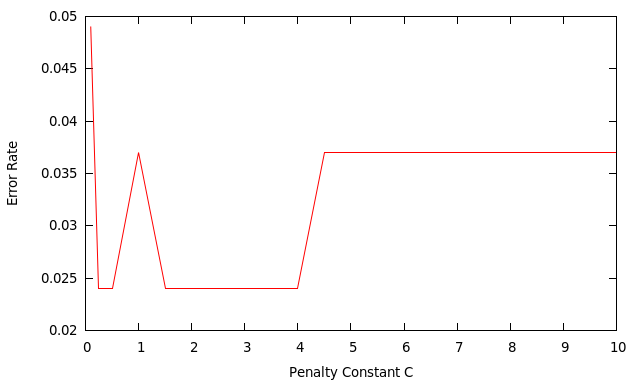
\includegraphics[width=0.9\textwidth]{radial_c_vs_error_rate.png}
\caption{Dual Radial Penality Constant Versus Error Rate}
\end{figure}

\begin{table}\label{table4}
\caption{Dual Radial Digit 3 vs 6 Error}
\begin{center}
\begin{tabular}{llcc}
\toprule
Data Set & Error & \multicolumn{2}{c}{95\% Confidence Interval} \\
\cmidrule(r){3-4}
& & Lower Bound & Upper Bound \\
\midrule
Training & 0.000 & 0.000 & 0.000 \\
Testing & 0.024 & -0.009 & 0.058 \\
\bottomrule
\end{tabular}
\end{center}
\end{table}

Table \ref{table4} indicates that the dual radial SVM classifier perfectly classified the training data set and achieved a \(0.024\) misclassification error rate for the testing data set for digits ''3`` and ''6``. This means that the radial and polynomial kernels actually performed identically well (but better than the dot product kernel machine). The polynomial kernel was chosen for the full problem.

\section{All Digits Polynomial Kernel}\label{full1}

Because of the size of the full classification problem, the ten hyperplanes (classifying each digit versus all others) were calculated using the NEOS server. The following is an example output from AMPL for the model defining the hyperplane separating digit ''9`` from other digits.

\begin{verbatim}

*************************************************************

   NEOS Server Version 5.0
   Job#     : 322513
   Password : ZDMlRVXE
   Solver   : nco:LOQO:AMPL
   Start    : 2012-10-13 15:37:19
   End      : 2012-10-13 15:38:32
   Host     : neos-4.chtc.wisc.edu

   Disclaimer:

   This information is provided without any express or
   implied warranty. In particular, there is no warranty
   of any kind concerning the fitness of this
   information  for any particular purpose.
*************************************************************
Job 322513 sent to neos-4.chtc.wisc.edu
password: ZDMlRVXE
---------- Begin Solver Output -----------
Executing /opt/neos/Drivers/loqo-ampl/loqo-driver.py at time: 2012-10-13 20:40:06.404104
File exists
You are using the solver loqo.

%% YOUR COMMENTS %%%%%%%%%%%%%%%%%%%%%%%
Digit 9
%%%%%%%%%%%%%%%%%%%%%%%%%%%%%%%%%%%%%%%%
Executing AMPL.
processing data.
processing commands.

930 variables, all nonlinear
1 constraint, all linear; 930 nonzeros
	1 equality constraint
1 nonlinear objective; 930 nonzeros.

LOQO 6.07: optimal solution (38 QP iterations, 112 evaluations)
primal objective 11434.38476
  dual objective 11434.3848
a [*] :=
  1   3.85436e-08   234   1.05483e-08   467   2.41951e-08   700  18.4227
  2   2.33818e-08   235   3.78196e-08   468  19.8573        701   4.7727e-08
  3   2.91404e-08   236   2.26497e-08   469   3.67114e-08   702   1.25251e-07
  4   5.71453       237   1.5172        470   6.27438e-07   703   3.03899e-08
  5   1.38018e-08   238   3.43765e-08   471   2.72169e-08   704 100
  6   7.05322       239   2.63027e-08   472   6.32506e-08   705   4.71152e-08
  7   2.3794e-08    240   1.57388e-08   473   3.68133e-08   706   1.5501e-07
  8   4.18764e-08   241   1.36029e-08   474   0.353602      707   2.60628e-08
  9   2.11997e-06   242   7.46301e-09   475   6.93911e-07   708   4.67655e-08
 10   5.60904e-08   243   5.82155e-09   476   1.47011e-08   709   4.23368e-08
 11   7.94764e-08   244   3.72253e-08   477   3.08854e-08   710 100
 12   3.58911e-08   245   9.042e-07     478  17.6082        711   2.41813e-07
 13   2.96835e-08   246   6.70782e-08   479   1.77021e-08   712  75.9297
 14   1.61716e-08   247   1.04641e-07   480   7.07884e-08   713   4.09782e-07
 15   1.47334e-07   248   2.6709e-08    481   6.68e-08      714   3.00134e-07
 16  29.3529        249   2.59011e-08   482   6.71728e-08   715   2.32582e-07
 17   9.64202e-08   250   7.87914e-08   483   3.86652e-08   716  18.5722
 18   3.38414e-08   251   8.84796e-08   484   6.63917e-08   717   6.01327e-08
 19   1.95048e-07   252   2.0955e-08    485   3.57116       718   2.26718e-07
 20   5.72279       253   1.57393e-08   486   8.43447e-08   719   2.79273e-08
 21   1.90208e-08   254   1.94778e-08   487   1.25587e-08   720   1.85065e-08
 22   2.05563e-08   255   2.05139e-08   488   5.93334e-08   721   7.0089
 23   2.22771e-07   256   5.84025e-09   489  36.5089        722   1.12219e-08
 24   6.59432e-08   257   8.92567e-09   490   2.439e-08     723   5.0506e-08
 25  87.9023        258   1.17714e-08   491   6.27438e-07   724   1.69498e-07
 26  54.8041        259   9.49884e-09   492   5.93334e-08   725 100
 27   1.39902e-06   260   9.14694e-09   493   3.72785e-08   726  13.7361
 28   0.000112796   261   2.53348e-08   494   9.11471e-08   727   4.73843e-08
 29   3.49784e-08   262   5.68235e-06   495   1.351e-07     728   8.65427
 30   3.49784e-08   263   3.99734e-08   496   3.1964e-08    729   2.41812e-08
 31   1.91778e-08   264   1.27274e-08   497   0.517183      730  51.0242
 32   5.77159e-08   265   1.44707e-08   498   3.4741e-08    731   8.55205e-08
 33   6.71962e-08   266   1.99829e-08   499   2.01095e-08   732   5.28158e-08
 34   4.73067e-08   267   3.90531e-08   500   4.46076e-08   733   3.55383e-08
 35   1.42603e-08   268   1.41763e-07   501   1.37996e-07   734   1.37807e-06
 36   1.7283e-08    269   6.40695e-08   502   7.66502e-08   735  40.0125
 37   2.86341e-08   270   2.03313e-08   503   9.57023e-09   736   3.15026e-08
 38   3.35671e-08   271   1.36457e-06   504   1.22933e-08   737   6.20972e-08
 39   6.37693e-08   272   2.20462e-08   505   9.57944e-09   738   3.01406e-08
 40   8.31286e-08   273   2.03325e-08   506   8.39667e-09   739  12.0501
 41   3.12044e-08   274   2.16373e-08   507   3.35393e-08   740   9.35406e-08
 42   3.12408e-08   275   6.13271e-08   508   5.49397e-08   741   6.73344e-08
 43   1.59441e-08   276   1.20099e-08   509  15.1377        742   2.2836e-07
 44   4.5707e-08    277  28.6054        510   2.33238e-08   743   6.32906e-08
 45   2.4491e-08    278   1.45522e-08   511   1.49538e-08   744  24.7776
 46   3.98829e-08   279   1.30016e-08   512   1.47931e-08   745   4.46246e-08
 47   3.0174e-08    280  42.4313        513   8.93877e-09   746   1.59093e-08
 48   2.16635e-08   281   2.49875e-08   514   2.06621e-08   747   1.87348e-08
 49   2.99249e-08   282   3.58647e-08   515   3.76778e-08   748   8.29901e-09
 50   4.79835e-08   283  31.6708        516   9.17331e-08   749   9.35097e-09
 51   3.10036e-08   284   1.27302e-08   517   2.03913e-08   750   6.06604e-08
 52   4.69671e-08   285   1.63198e-08   518   6.81754e-08   751   4.45899e-08
 53  31.0034        286   4.8192e-08    519   6.72317e-07   752   2.68031e-08
 54   1.65889e-07   287   1.47451e-08   520   3.23831e-08   753  63.8287
 55   1.42681e-08   288   2.21206e-08   521  12.4197        754   5.39902e-08
 56   2.96805e-08   289  10.9079        522   5.6307e-08    755   1.65101e-08
 57   2.59437e-08   290   6.1962e-08    523   2.13867e-08   756   1.7601e-08
 58   2.8481e-08    291   4.4776e-08    524   1.09866e-07   757   6.68351e-08
 59   1.32139e-08   292   3.91747e-08   525   5.44633e-08   758   2.26889e-07
 60   3.67646e-08   293   2.34207e-08   526   1.2047e-07    759   5.46958e-08
 61  10.4148        294   4.33321e-08   527   1.69765e-08   760   4.07936e-08
 62   3.26254e-08   295   2.37069e-08   528  37.345         761   2.70216e-08
 63   8.23382e-08   296   2.44745e-08   529   5.21229       762   2.53618e-08
 64   5.23811e-08   297   2.47458e-08   530  29.8444        763  30.3426
 65   1.34593e-07   298   4.81607e-08   531   2.354e-08     764   2.88914e-08
 66   3.82011e-08   299   5.47056e-08   532   1.40526e-08   765   3.68228e-08
 67   5.96743e-08   300   2.32321e-08   533   4.2098e-08    766   3.29692e-08
 68   3.26868e-08   301   1.42289e-07   534  70.0837        767   7.22012e-08
 69   2.96036e-08   302   3.37744e-08   535   9.13876e-09   768  98.6327
 70   3.44339e-08   303   4.36211e-08   536   8.75874e-09   769   5.68451e-08
 71   2.76635e-08   304   2.60821e-08   537   2.73822e-07   770  27.4658
 72   4.66116e-08   305   2.7947e-08    538   1.74901e-06   771   5.39902e-08
 73   3.88695e-08   306   0.175107      539  72.0049        772   1.91334e-07
 74   5.16296e-08   307   2.03907e-07   540   2.56229e-08   773   5.58844e-08
 75   1.05899e-07   308   9.98471       541   5.09203e-08   774   2.94872e-08
 76   2.16298e-08   309   5.19411e-08   542   2.37141e-07   775  39.8487
 77   3.82416e-08   310   2.503e-08     543   1.33879e-08   776  80.8929
 78   1.76589e-08   311   1.87832e-08   544   2.4519e-06    777   1.59144e-08
 79   1.22373e-07   312   4.95507e-07   545   2.31918e-08   778   1.31574e-07
 80   4.0689e-06    313  28.4913        546   5.18578       779 100
 81   9.3058e-08    314   1.34279e-08   547   3.33864e-08   780   1.63384e-08
 82   4.28731e-08   315  20.7138        548   9.4663e-08    781   9.08261e-08
 83   7.14995e-08   316   1.42517e-08   549   2.57318e-08   782   4.12276e-08
 84   6.92773e-08   317  55.0932        550   2.735e-08     783   1.72565e-08
 85   2.54506e-08   318   7.24769e-09   551   2.10952e-08   784   1.28544e-07
 86   1.23417e-07   319   6.07053e-09   552 100             785  28.4671
 87   3.87228e-08   320   1.44993e-08   553  14.6866        786   3.5382e-08
 88   5.19699e-07   321   1.14318e-08   554  51.7308        787   1.11575e-08
 89   9.56465e-08   322   9.4297e-08    555  20.6688        788   1.1578e-08
 90   2.26018e-08   323   2.15618e-08   556   4.88641       789   9.90283e-09
 91   4.57081e-08   324   3.67134       557   8.95684e-08   790  13.6659
 92   3.4908e-08    325   1.55879e-08   558   7.12494e-08   791   6.051e-08
 93   1.31665       326   4.23239e-08   559   1.73796e-08   792   1.25531e-08
 94   1.84953e-07   327   1.12298e-08   560   3.04043e-08   793   8.28471e-09
 95   1.04024e-06   328   1.35997e-08   561   1.73769e-08   794   1.5172
 96   1.12866e-07   329   1.47122e-08   562   1.66743e-08   795   1.05734e-07
 97 100             330   0.637703      563   1.08723e-08   796   5.1897e-08
 98 100             331   8.05242e-08   564  19.1401        797   1.27939e-07
 99   2.58436e-08   332   4.10269e-08   565   1.21165e-08   798  11.4375
100   6.19801e-08   333   4.22526e-08   566   6.72943e-09   799   2.77049e-08
101   5.04257e-08   334   2.51607e-06   567   3.20842e-08   800   2.38846e-08
102   1.11166e-07   335   7.09107e-09   568   1.71234e-08   801   1.34923e-08
103   4.89188e-08   336   1.54768e-08   569   3.9541e-08    802  43.5287
104   4.62787e-07   337   9.31113e-09   570   1.73492e-08   803   4.02628e-08
105   1.28079e-07   338  26.5263        571   1.95366e-08   804   1.95869e-07
106  32.7716        339   8.15323e-08   572   1.2651e-08    805  33.8906
107   8.49446e-08   340   3.67562e-08   573   2.58757e-08   806   5.76479e-08
108   7.58618e-08   341  76.5891        574   5.1005e-08    807   2.80831e-08
109   1.83277e-07   342   2.86211e-08   575  75.4697        808   5.47591e-08
110   1.28079e-07   343   5.01951e-08   576   4.62622e-08   809   5.33724e-08
111   1.84953e-07   344   1.7571e-06    577   3.77306e-08   810   2.58255e-08
112   1.4635e-07    345   2.66057e-08   578   2.72308e-08   811   6.94816
113   1.37781e-07   346   2.23407e-08   579   2.23639e-08   812   1.10208e-08
114   1.37781e-07   347 100             580   2.14761e-07   813  32.9226
115   8.79441e-06   348  50.2192        581   3.03802e-08   814  24.7422
116   3.71935e-06   349   2.44918e-08   582   1.12664e-08   815  38.3727
117  11.9145        350   1.06024e-08   583   3.63946e-08   816  88.5056
118   3.38051e-07   351   1.2334e-08    584   8.5299e-08    817  18.4125
119   3.38051e-07   352   1.77221e-08   585   1.99742e-08   818   1.84441e-08
120   3.87516e-07   353   1.21483e-08   586   4.24965e-08   819   2.72733e-08
121   1.84953e-07   354   1.26128e-08   587   1.81451e-08   820   1.69932e-08
122   1.84953e-07   355   3.02331e-08   588   1.8592e-08    821   1.03389e-08
123   3.87516e-07   356   5.59393e-08   589   1.65819e-08   822   1.22589e-08
124   1.28079e-07   357   1.35925e-08   590   1.91717e-08   823   9.70715e-07
125  47.6849        358   1.43543e-08   591   4.3219e-08    824   6.40877e-08
126   2.80476e-07   359   3.23171e-08   592   1.76876e-08   825   1.1659e-08
127   1.3426e-07    360   3.06975       593   4.00608e-08   826   1.97428e-08
128   1.64991e-06   361  18.6384        594   8.40152e-08   827  64.2707
129   1.74233e-08   362   6.1922        595   2.79754e-08   828  10.215
130   2.07108e-08   363  78.9539        596   3.14686e-08   829   1.33594e-08
131   4.8475e-08    364   6.41814e-08   597   4.74008e-08   830   2.33468e-08
132   2.3094e-07    365   1.75939e-07   598   7.67663e-09   831   2.88313e-08
133   1.28079e-07   366 100             599   7.0626e-09    832   1.28804e-07
134   9.09461e-08   367   1.04522e-07   600   1.45123e-08   833   2.3411e-07
135   5.04488e-08   368   3.25504e-06   601   4.9579e-08    834   6.58494e-09
136   5.65006e-08   369   2.13498e-08   602   2.21507e-08   835   8.49227e-09
137  54.0187        370   2.90897e-08   603   1.6761e-08    836  45.5049
138   1.04783e-07   371   2.03738e-08   604   2.26405e-08   837   1.58665e-07
139   4.32154e-08   372   4.57929e-08   605   1.75805e-08   838 100
140   3.27177e-08   373  57.4036        606   7.66174e-09   839 100
141  19.8018        374  80.5618        607   8.65486e-09   840  75.5841
142   1.65822e-08   375   3.5791e-08    608   2.87527e-08   841 100
143   1.28079e-07   376   5.8046e-07    609   8.11502e-08   842   1.75801
144   1.36136e-07   377   7.80957       610   1.57627e-08   843  68.7307
145   4.42464       378 100             611   2.81648e-08   844 100
146   4.42464       379   2.3624e-08    612   1.21696e-08   845 100
147   2.25185       380  21.3358        613   9.14794e-09   846  96.2966
148   2.12267e-08   381   3.34692       614   1.50895e-08   847 100
149   1.97217e-06   382   2.43224e-08   615   6.377e-08     848 100
150   9.48228e-08   383  19.7623        616   1.30377e-08   849 100
151   6.07154e-08   384   1.7773e-08    617   7.55313e-09   850 100
152   3.28686e-07   385   5.95064e-08   618   3.77044e-08   851 100
153   3.38051e-07   386 100             619   4.07183e-08   852 100
154   2.12024e-07   387  78.8262        620   1.36882e-07   853 100
155   4.22157e-08   388 100             621   2.92982e-08   854 100
156   1.5468e-07    389 100             622   4.50559e-08   855 100
157   3.87516e-07   390 100             623   2.82885e-08   856 100
158   3.87516e-07   391 100             624   2.07988e-08   857   1.04596e-08
159   1.3831e-06    392  56.4784        625   1.77983e-08   858 100
160   4.79717e-07   393 100             626   1.9582e-08    859 100
161  49.0921        394 100             627   5.68782e-08   860 100
162   6.13672e-08   395   8.20026e-06   628   8.64019e-09   861 100
163 100             396   6.71269e-08   629   7.87476e-09   862 100
164   1.5468e-07    397   3.38579e-08   630   5.66023e-07   863 100
165   1.07222e-07   398   5.06326e-07   631   1.62355e-07   864 100
166   2.82807e-08   399   7.6426        632   1.09438e-08   865 100
167   5.14082e-08   400   3.06399e-07   633   1.14288e-08   866 100
168   6.5556e-08    401   6.73477e-08   634   6.08075e-08   867 100
169   1.99022e-07   402  10.9476        635   4.48262e-08   868  95.0609
170   1.55763e-07   403  10.2913        636   1.03931e-08   869  80.4406
171   9.57792e-08   404  55.463         637   4.10875e-07   870   1.7725e-08
172   1.77256e-07   405  55.463         638   1.45356e-08   871 100
173   1.28079e-07   406 100             639   9.97896e-09   872 100
174   1.28079e-07   407 100             640   7.40196e-08   873 100
175   1.5468e-07    408   5.92706e-08   641   4.53697e-08   874 100
176   3.76924e-07   409  16.7006        642   1.34486e-08   875   2.971e-08
177   7.17095e-08   410  95.4299        643   2.33863e-08   876 100
178   4.93011e-08   411  88.144         644   1.3594e-08    877  16.1071
179   4.09529e-08   412   2.30298e-07   645   1.98503e-08   878   1.77163e-08
180   4.39501e-08   413   2.48605e-08   646   3.63608e-08   879  77.6427
181   1.5468e-07    414 100             647   4.307e-08     880 100
182   1.84953e-07   415  44.7108        648   1.48356e-08   881 100
183   1.54054e-07   416 100             649   1.35881e-08   882 100
184   1.84953e-07   417 100             650   3.11491e-08   883   1.62455e-07
185   1.28079e-07   418  97.1921        651   1.15842e-08   884  29.8817
186   4.62787e-07   419  97.1921        652   6.74876       885 100
187   1.9273e-08    420  32.7374        653   9.52087e-08   886  71.0149
188   1.3828e-08    421  71.4222        654   7.36822       887 100
189   2.82894e-08   422   3.45104e-08   655   1.99873e-07   888 100
190   1.4286e-08    423   3.89171e-07   656   7.56789e-08   889 100
191   1.50038e-08   424   1.17789e-08   657   8.36207e-08   890 100
192   2.22259e-08   425  47.6717        658   4.73264e-08   891 100
193   2.30676e-08   426 100             659   9.26251       892 100
194   1.53127e-08   427   8.29243e-08   660  12.6838        893  56.862
195   1.63587e-08   428   3.64277e-08   661   1.7387e-07    894 100
196   6.7986e-08    429   3.52821e-08   662  86.5115        895 100
197   2.43525e-08   430   8.84289       663   1.08575e-07   896 100
198   5.32598e-08   431   7.09862e-08   664  91.7738        897 100
199   3.43494       432   6.81808e-07   665  35.1577        898 100
200   1.46164e-07   433   5.45843e-08   666  14.0485        899 100
201   7.88909e-08   434   2.80329e-08   667  84.9883        900 100
202   2.62519e-08   435   1.17527e-08   668   5.00021e-07   901 100
203   3.36905e-08   436   4.9578e-08    669   9.70082e-08   902 100
204   5.10527e-08   437   2.68206e-08   670   7.58446e-08   903 100
205   2.45367e-08   438   2.24286e-05   671  58.0712        904 100
206   3.07102e-08   439   7.62233e-07   672   6.29752e-08   905 100
207  11.3626        440   6.63937e-08   673  35.4276        906 100
208   4.64869e-08   441   2.48883e-08   674   4.33488e-06   907   3.30393
209   2.03694e-08   442 100             675   5.56842e-08   908 100
210   1.92825e-08   443   3.54369e-08   676   2.95101e-08   909 100
211   1.02081e-07   444 100             677   2.95615e-08   910 100
212   1.40133e-08   445 100             678   1.70771e-08   911  60.9945
213  34.3667        446 100             679  32.1771        912  95.8192
214   6.60261e-08   447 100             680   7.1615e-08    913  43.4258
215   4.53354e-08   448  62.7717        681   3.36267e-07   914   1.50456e-07
216   5.08046e-08   449   3.3631e-08    682   5.90314e-08   915 100
217   6.234e-08     450   6.61826e-09   683   7.40521e-08   916  19.1198
218   8.34583e-09   451   1.96369e-08   684   9.2942e-08    917 100
219   1.91146e-08   452 100             685  10.7575        918  55.288
220   2.72102e-08   453   6.45754e-08   686  59.5014        919 100
221   1.2318e-08    454   7.66703e-07   687  19.0044        920 100
222   2.73081e-08   455   4.03601e-08   688   9.32704e-07   921 100
223   2.45947e-08   456   1.64845e-07   689   1.60998e-07   922 100
224   5.64483e-08   457  71.0304        690  82.9783        923 100
225   2.69912e-08   458   4.19629e-08   691   2.57498e-08   924 100
226   1.63384e-08   459   3.58107e-08   692   3.11657e-08   925 100
227   7.12442e-09   460  70.1068        693   9.5684        926 100
228   1.65566e-08   461 100             694   9.31443e-08   927 100
229   8.65693e-09   462   2.9108e-08    695   1.26076e-07   928   4.83518e-08
230   1.14368e-08   463   1.4836e-07    696   1.39693e-08   929   3.88496e-07
231   2.09631e-08   464   3.21062e-08   697  40.7794        930  36.1626
232   1.90661e-08   465   1.93438e-07   698  10.2959
233  18.3483        466   3.24508e-08   699   3.94902e-08
;

\end{verbatim}

The above results contain 155 support vectors from among the 930 input data elements. This relatively low percentage of the total input data elements suggests that the choice of \(C=100\) was a reasonable one. Calculating the \(b\) value for each support vectors verifies that we get the same value for each.

\begin{verbatim}

#alpha index, alpha value, calculated b
3 5.7145 1.070456954818
5 7.0532 1.070458003550
15 29.3529 1.070456917860
19 5.7228 1.070457321617
24 87.9023 1.070456625551
25 54.8041 1.070457086784
52 31.0034 1.070457811208
60 10.4148 1.070456139039
92 1.3167 1.070456399823
105 32.7716 1.070456500112
116 11.9145 1.070456581841
124 47.6849 1.070456477399
136 54.0187 1.070455837201
140 19.8018 1.070456446670
144 4.4246 1.070456433282
145 4.4246 1.070456433282
146 2.2519 1.070456667867
160 49.0921 1.070456525914
198 3.4349 1.070456384679
206 11.3626 1.070458249808
212 34.3667 1.070456498634
232 18.3483 1.070456385869
236 1.5172 1.070456647091
276 28.6054 1.070456057211
279 42.4313 1.070456639370
282 31.6708 1.070456735161
288 10.9079 1.070455501098
305 0.1751 1.070381117977
307 9.9847 1.070456389796
312 28.4913 1.070455653409
314 20.7138 1.070456614663
316 55.0932 1.070457995762
323 3.6713 1.070456015144
329 0.6377 1.070456248119
337 26.5263 1.070457614809
340 76.5891 1.070457006468
347 50.2192 1.070456808547
359 3.0698 1.070456029499
360 18.6384 1.070455919222
361 6.1922 1.070456396369
362 78.9539 1.070455745002
372 57.4036 1.070456414550
373 80.5618 1.070456775276
376 7.8096 1.070456150539
379 21.3358 1.070457653196
380 3.3469 1.070456700692
382 19.7623 1.070456114907
386 78.8262 1.070456183524
391 56.4784 1.070457004452
398 7.6426 1.070456665992
401 10.9476 1.070457026473
402 10.2913 1.070456211710
403 55.4630 1.070456494051
404 55.4630 1.070456494051
408 16.7006 1.070456330389
409 95.4299 1.070456683881
410 88.1440 1.070457111230
414 44.7108 1.070457330137
417 97.1921 1.070456082030
418 97.1921 1.070456082030
419 32.7374 1.070455447269
420 71.4222 1.070456351084
424 47.6717 1.070456308539
429 8.8429 1.070456125046
447 62.7717 1.070457240982
456 71.0304 1.070456527582
459 70.1068 1.070456765760
467 19.8573 1.070456469188
473 0.3536 1.070453295132
477 17.6082 1.070455989484
484 3.5712 1.070456784877
488 36.5089 1.070456801288
496 0.5172 1.070455405047
508 15.1377 1.070455287170
520 12.4197 1.070457034677
527 37.3450 1.070455997986
528 5.2123 1.070456714431
529 29.8444 1.070456600401
533 70.0837 1.070456363542
538 72.0049 1.070456247672
545 5.1858 1.070456556141
552 14.6866 1.070456764543
553 51.7308 1.070456424819
554 20.6688 1.070456232390
555 4.8864 1.070456320348
563 19.1401 1.070457944652
574 75.4697 1.070456477919
651 6.7488 1.070456447351
653 7.3682 1.070456680096
658 9.2625 1.070456497349
659 12.6838 1.070456515841
661 86.5115 1.070456481616
663 91.7738 1.070456456564
664 35.1577 1.070456411878
665 14.0485 1.070456610638
666 84.9883 1.070456200115
670 58.0712 1.070457679985
672 35.4276 1.070456687916
678 32.1771 1.070456718883
684 10.7575 1.070456253366
685 59.5014 1.070456122071
686 19.0044 1.070456369104
689 82.9783 1.070456075705
692 9.5684 1.070456764190
696 40.7794 1.070456801773
697 10.2959 1.070457073814
699 18.4227 1.070456614667
711 75.9297 1.070456463361
715 18.5722 1.070456524221
720 7.0089 1.070457290112
725 13.7361 1.070456591122
727 8.6543 1.070456620797
729 51.0242 1.070456358756
734 40.0125 1.070455959872
738 12.0501 1.070456449213
743 24.7776 1.070457480324
752 63.8287 1.070455529656
762 30.3426 1.070457621112
767 98.6327 1.070456496127
769 27.4658 1.070457317837
774 39.8487 1.070454592313
775 80.8929 1.070457578619
784 28.4671 1.070455676275
789 13.6659 1.070455131373
793 1.5172 1.070456647091
797 11.4375 1.070457837635
801 43.5287 1.070457748747
804 33.8906 1.070456243569
810 6.9482 1.070456603963
812 32.9226 1.070456314772
813 24.7422 1.070455201870
814 38.3727 1.070458871934
815 88.5056 1.070456433800
816 18.4125 1.070455626052
826 64.2707 1.070456508596
827 10.2150 1.070455437992
835 45.5049 1.070454735535
839 75.5841 1.070456811927
841 1.7580 1.070457939916
842 68.7307 1.070457902706
845 96.2966 1.070456418024
867 95.0609 1.070455977351
868 80.4406 1.070456095607
876 16.1071 1.070455674830
878 77.6427 1.070457079420
883 29.8817 1.070455733096
885 71.0149 1.070456266973
892 56.8620 1.070457034931
906 3.3039 1.070457104102
910 60.9945 1.070456691140
911 95.8192 1.070455688802
912 43.4258 1.070458233218
915 19.1198 1.070456181082
917 55.2880 1.070457362156
929 36.1626 1.070455834797

\end{verbatim}

\begin{table}\label{tablefull}
\caption{Dual Polynomial All Digits Error}
\begin{center}
\begin{tabular}{llcc}
\toprule
Data Set & Error & \multicolumn{2}{c}{95\% Confidence Interval} \\
\cmidrule(r){3-4}
& & Lower Bound & Upper Bound \\
\midrule
Training & 0.029 & 0.018 & 0.040 \\
Testing & 0.200 & -0.161 & 0.239 \\
\bottomrule
\end{tabular}
\end{center}
\end{table}

As indicated in Table \ref{tablefull}, the overall testing misclassification error achieved by the polynomial SVM classifier was \(0.2\). This is significantly better than the \(0.9\) misclassification error that we would expect to achieve by random guessing.

\end{document}
